% questions.tex —— 2008 年·普通高等学校招生考试·湖北卷·文科 · 题目内容片段（无答案）
% 由 tools/generate_projects.py 依来源总账自 2008/2008_数学真题_湖北文_试题.md 生成，勿手改（改源 MD 后重跑）


\gkpart{一、选择题}

\begin{question}
\gkti{1}设 $\boldsymbol a=(1,-2)$，$\boldsymbol b=(-3,4)$，$\boldsymbol c=(3,2)$，则 $(\boldsymbol a+2\boldsymbol b)\cdot\boldsymbol c=$（　）

（A）$(-15,12)$

（B）$0$

（C）$-3$

（D）$-11$

\end{question}
\begin{question}
\gkti{2}$\left(2x^3-\dfrac1{2x^2}\right)^{10}$ 的展开式中常数项是（　）

（A）$210$

（B）$\dfrac{105}2$

（C）$\dfrac14$

（D）$-105$

\end{question}
\begin{question}
\gkti{3}若集合 $P=\{1,2,3,4\}$，$Q=\{x\mid 0<x<5,\ x\in\mathbf R\}$，则（　）

（A）“$x\in P$”是“$x\in Q$”的充分条件但不是必要条件

（B）“$x\in P$”是“$x\in Q$”的必要条件但不是充分条件

（C）“$x\in P$”是“$x\in Q$”的充要条件

（D）“$x\in P$”既不是“$x\in Q$”的充分条件也不是“$x\in Q$”的必要条件

\end{question}
\begin{question}
\gkti{4}用与球心距离为 $1$ 的平面去截球，所得的截面面积为 $\pi$，则球的体积为（　）

（A）$\dfrac{8\pi}3$

（B）$\dfrac{8\sqrt2\pi}3$

（C）$8\sqrt2\pi$

（D）$\dfrac{32\pi}3$

\Needspace{0.4\textheight}
\end{question}
\begin{question}
\gkti{5}在平面直角坐标系 $xOy$ 中，满足不等式组 $\begin{cases}|x|\leqslant|y|,\\ |x|<1\end{cases}$ 的点 $(x,y)$ 的集合用阴影表示为下列图中的（　）
\nopagebreak[4]
\begin{center}% 2008 年湖北卷文科第 5 题：不等式组 |x|<=|y|、|x|<1 所表示区域的四个候选图。
% 来源 PDF：gaokaomath-src/普通高考/2008/2008湖北文.pdf
% SHA-256：e097163e244cb8f03775ac7ff2e344ef85471e91ecc717d23698a0fb01e76963
% 原页：2008湖北文.pdf 第 1 页（A3 三栏）第 1 栏，书页码 451。
% 绘制依据：四个候选按原页排成 2×2——
%   (A) |x|<=|y| 且 |y|<=1（上下两个三角，横向虚线 y=±1）；
%   (B) y>=|x| 且 |x|<1（上方楔形，竖向虚线 x=±1）；
%   (C) |x|<=|y| 且 |x|<1（上下两个楔形，竖向虚线 x=±1）——即题设区域；
%   (D) |y|<=|x| 且 |x|<1（左右两个楔形，竖向虚线 x=±1）。
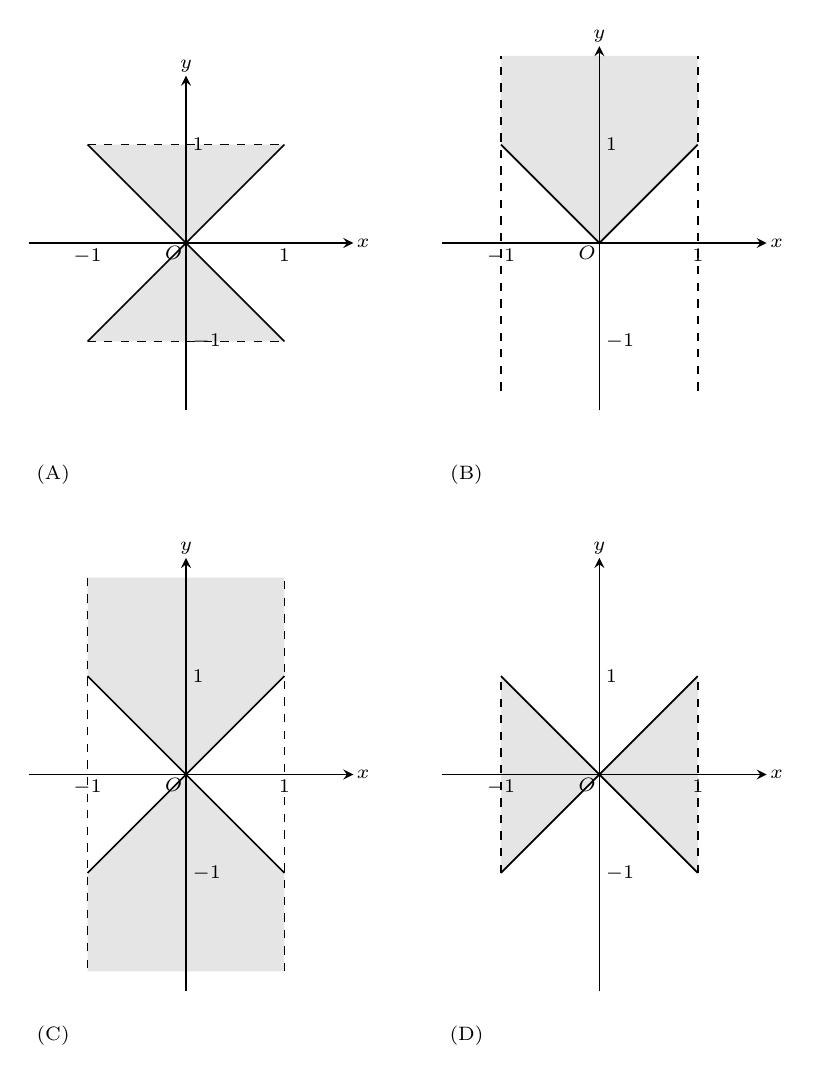
\begin{tikzpicture}[x=1.25cm, y=1.25cm, semithick, font=\scriptsize,
  every node/.style={inner sep=1.0pt}]

  % ---------- (A) |x|<=|y|<=1 ----------
  \begin{scope}[shift={(0,0)}]
    \fill[gray!20] (-1,1) -- (0,0) -- (1,1) -- cycle;
    \fill[gray!20] (-1,-1) -- (0,0) -- (1,-1) -- cycle;
    \draw[->,>=stealth] (-1.6,0) -- (1.7,0) node[right] {$x$};
    \draw[->,>=stealth] (0,-1.7) -- (0,1.7) node[above] {$y$};
    \node[below left] at (0,0) {$O$};
    \draw[dashed] (-1,1) -- (1,1);
    \draw[dashed] (-1,-1) -- (1,-1);
    \draw (-1,1) -- (0,0) -- (1,1);
    \draw (-1,-1) -- (0,0) -- (1,-1);
    \node[below] at (-1,-0.02) {$-1$};
    \node[below] at (1,-0.02) {$1$};
    \node[right] at (0.03,1) {$1$};
    \node[right] at (0.03,-1) {$-1$};
    \node at (-1.35,-2.35) {(A)};
  \end{scope}

  % ---------- (B) y>=|x|, |x|<1 ----------
  \begin{scope}[shift={(4.2,0)}]
    \fill[gray!20] (-1,1) -- (-1,1.9) -- (1,1.9) -- (1,1) -- (0,0) -- cycle;
    \draw[->,>=stealth] (-1.6,0) -- (1.7,0) node[right] {$x$};
    \draw[->,>=stealth] (0,-1.7) -- (0,2.0) node[above] {$y$};
    \node[below left] at (0,0) {$O$};
    \draw[dashed] (-1,-1.5) -- (-1,1.9);
    \draw[dashed] (1,-1.5) -- (1,1.9);
    \draw (-1,1) -- (0,0) -- (1,1);
    \node[below] at (-1,-0.02) {$-1$};
    \node[below] at (1,-0.02) {$1$};
    \node[right] at (0.03,1) {$1$};
    \node[right] at (0.03,-1) {$-1$};
    \node at (-1.35,-2.35) {(B)};
  \end{scope}

  % ---------- (C) |x|<=|y|, |x|<1 ----------
  \begin{scope}[shift={(0,-5.4)}]
    \fill[gray!20] (-1,1) -- (-1,2.0) -- (1,2.0) -- (1,1) -- (0,0) -- cycle;
    \fill[gray!20] (-1,-1) -- (-1,-2.0) -- (1,-2.0) -- (1,-1) -- (0,0) -- cycle;
    \draw[->,>=stealth] (-1.6,0) -- (1.7,0) node[right] {$x$};
    \draw[->,>=stealth] (0,-2.2) -- (0,2.2) node[above] {$y$};
    \node[below left] at (0,0) {$O$};
    \draw[dashed] (-1,2.0) -- (-1,-2.0);
    \draw[dashed] (1,-2.0) -- (1,2.0);
    \draw (-1,1) -- (0,0) -- (1,1);
    \draw (-1,-1) -- (0,0) -- (1,-1);
    \node[below] at (-1,-0.02) {$-1$};
    \node[below] at (1,-0.02) {$1$};
    \node[right] at (0.03,1) {$1$};
    \node[right] at (0.03,-1) {$-1$};
    \node at (-1.35,-2.65) {(C)};
  \end{scope}

  % ---------- (D) |y|<=|x|, |x|<1 ----------
  \begin{scope}[shift={(4.2,-5.4)}]
    \fill[gray!20] (-1,1) -- (-1,-1) -- (0,0) -- cycle;
    \fill[gray!20] (1,1) -- (1,-1) -- (0,0) -- cycle;
    \draw[->,>=stealth] (-1.6,0) -- (1.7,0) node[right] {$x$};
    \draw[->,>=stealth] (0,-2.2) -- (0,2.2) node[above] {$y$};
    \node[below left] at (0,0) {$O$};
    \draw[dashed] (-1,-1) -- (-1,1);
    \draw[dashed] (1,-1) -- (1,1);
    \draw (-1,1) -- (0,0) -- (-1,-1);
    \draw (1,1) -- (0,0) -- (1,-1);
    \node[below] at (-1,-0.02) {$-1$};
    \node[below] at (1,-0.02) {$1$};
    \node[right] at (0.03,1) {$1$};
    \node[right] at (0.03,-1) {$-1$};
    \node at (-1.35,-2.65) {(D)};
  \end{scope}
\end{tikzpicture}
\end{center}
\nopagebreak[4]
\end{question}
\begin{question}
\gkti{6}已知 $f(x)$ 在 $\mathbf R$ 上是奇函数，且 $f(x+4)=f(x)$，当 $x\in(0,2)$ 时，$f(x)=2x^2$，则 $f(7)=$（　）

（A）$-2$

（B）$2$

（C）$-98$

（D）$98$

\end{question}
\begin{question}
\gkti{7}将函数 $y=\sin(x-\theta)$ 的图象 $F$ 向右平移 $\dfrac{\pi}3$ 个单位长度得到图象 $F'$，若 $F'$ 的一条对称轴是直线 $x=\dfrac{\pi}4$，则 $\theta$ 的一个可能取值是（　）

（A）$\dfrac5{12}\pi$

（B）$-\dfrac5{12}\pi$

（C）$\dfrac{11}{12}\pi$

（D）$-\dfrac{11}{12}\pi$

\end{question}
\begin{question}
\gkti{8}函数 $f(x)=\dfrac1x\ln\left(\sqrt{x^2-3x+2}+\sqrt{-x^2-3x+4}\right)$ 的定义域为（　）

（A）$(-\infty,-4]\cup[2,+\infty)$

（B）$(-4,0)\cup(0,1)$

（C）$[-4,0)\cup(0,1]$

（D）$[-4,0)\cup(0,1)$

\end{question}
\begin{question}
\gkti{9}从 $5$ 名男生和 $5$ 名女生中选 $3$ 人组队参加某集体项目的比赛，其中至少有一名女生入选的组队方案数为（　）

（A）$100$

（B）$110$

（C）$120$

（D）$180$

\Needspace{0.4\textheight}
\end{question}
\begin{question}
\gkti{10}如图所示，“嫦娥一号”探月卫星沿地月转移轨道飞向月球，在月球附近一点 $P$ 轨进入以月球球心 $F$ 为一个焦点的椭圆轨道 I 绕月飞行，之后卫星在 $P$ 点第二次变轨进入仍以 $F$ 为一个焦点的椭圆轨道 II 绕月飞行，最终卫星在 $P$ 点第三次变轨进入以 $F$ 为圆心的圆形轨道 III 绕月飞行，若用 $2c_1$ 和 $2c_2$ 分别表示椭圆轨道 I 和 II 的焦距，用 $2a_1$ 和 $2a_2$ 分别表示椭圆轨道 I 和 II 的长轴的长，给出下列式子：

① $a_1+c_1=a_2+c_2$；② $a_1-c_1=a_2-c_2$；③ $c_1a_2>a_1c_2$；④ $\dfrac{c_1}{a_1}<\dfrac{c_2}{a_2}$。

其中正确式子的序号是（　）
\nopagebreak[4]
\begin{center}% 2008 年湖北卷文科第 10 题：三条以 F 为焦点的轨道（椭圆 I、II 与圆 III）在 P 点相切。
% 来源 PDF：gaokaomath-src/普通高考/2008/2008湖北文.pdf
% SHA-256：e097163e244cb8f03775ac7ff2e344ef85471e91ecc717d23698a0fb01e76963
% 原页：2008湖北文.pdf 第 1 页（A3 三栏）第 2 栏，书页码 451。
% 绘制依据：按原页 P 在最上方、F 在其下方，三条轨道在 P 处相切：椭圆 I 最大、II 次之，
%   圆 III 以 F 为圆心；贯穿 P、F 的对称轴用虚线，轨道编号标在右侧。
%   取 |PF|=1.5：椭圆 I 的 a=2.4、c=0.9；椭圆 II 的 a=1.9、c=0.4；圆 III 半径 1.5。
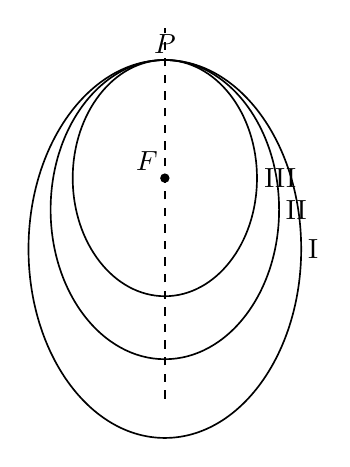
\begin{tikzpicture}[x=0.78cm, y=1.0cm, semithick, every node/.style={inner sep=1.3pt}]
  % 对称轴
  \draw[dashed] (0,-1.7) -- (0,3.0);

  % 椭圆 I：中心 (0,0.2)，半长轴 2.4、半短轴 2.22
  \draw (0,0.2) ellipse [x radius=2.22, y radius=2.4];
  % 椭圆 II：中心 (0,0.7)，半长轴 1.9、半短轴 1.86
  \draw (0,0.7) ellipse [x radius=1.86, y radius=1.9];
  % 圆 III：圆心 F(0,1.1)，半径 1.5
  \draw (0,1.1) circle [radius=1.5];

  % 焦点与切点
  \fill (0,1.1) circle (1.7pt);
  \node[above left=1pt] at (0,1.1) {$F$};
  \node[above] at (0,2.62) {$P$};

  \node[right] at (2.26,0.20) {I};
  \node[right] at (1.90,0.70) {II};
  \node[right] at (1.55,1.10) {III};
\end{tikzpicture}
\end{center}
\nopagebreak[4]
（A）①③

（B）②③

（C）①④

（D）②④

\end{question}
\gkpart{二、填空题}

\begin{question}
\gkti{11}一个公司共有 $1000$ 名员工，下设一些部门，要采用分层抽样方法从全体员工中抽取一个容量为 $50$ 的样本，已知某部门有 $200$ 名员工，那么从该部门抽取的员工人数是\gkblank{}。

\end{question}
\begin{question}
\gkti{12}在 $\triangle ABC$ 中，$a$，$b$，$c$ 分别是角 $A$，$B$，$C$ 所对的边，已知 $a=\sqrt3$，$b=3$，$c=30^\circ$，则 $A=$\gkblank{}。

\end{question}
\begin{question}
\gkti{13}方程 $2^{-x}+x^2=3$ 的实数解的个数为\gkblank{}。

\end{question}
\begin{question}
\gkti{14}明天上午李明要参加奥运志愿者活动，为了准时起床，他用甲、乙两个闹钟叫醒自己。假设甲闹钟准时响的概率是 $0.80$，乙闹钟准时响的概率是 $0.90$，则两个闹钟至少有一准时响的概率是\gkblank{}。

\end{question}
\begin{question}
\gkti{15}圆 $C$：$\begin{cases}x=3+4\cos\theta,\\ y=-2+4\sin\theta,\end{cases}$（$\theta$ 为参数）的圆心坐标为\gkblank{}，和圆 $C$ 关于直线 $x-y=0$ 对称的圆 $C'$ 的普通方程是\gkblank{}。

\end{question}
\gkpart{三、解答题}

\begin{question}
\gkti{16}已知函数 $f(x)=\sin\dfrac x2\cos\dfrac x2+\cos^2\dfrac x2-2$。

（1）将函数 $f(x)$ 化简成 $A\sin(\omega x+\varphi)+B$（$A>0$，$\omega>0$，$\varphi\in[0,2\pi)$）的形式，并指出 $f(x)$ 的周期；

（2）求函数 $f(x)$ 在 $\left[\pi,\dfrac{17\pi}{12}\right]$ 上的最大值和最小值。

\end{question}
\begin{question}
\gkti{17}已知函数 $f(x)=x^3+mx^2-m^2x+1$（$m$ 为常数，且 $m>0$）有极大值 $9$。

（1）求 $m$ 的值；

（2）若斜率为 $-5$ 的直线是曲线 $y=f(x)$ 的切线，求此直线方程。

\Needspace{0.4\textheight}
\end{question}
\begin{question}
\gkti{18}如图，在直三棱柱 $ABC-A_1B_1C_1$ 中，平面 $A_1BC\perp$ 侧面 $A_1ABB_1$。

（1）求证：$AB\perp BC$；

（2）若 $AA_1=AC=a$，直线 $AC$ 与平面 $A_1BC$ 所成的角为 $\theta$，二面角 $A_1-BC-A$ 的大小为 $\varphi$，求证：$\theta+\varphi=\dfrac{\pi}2$。
\nopagebreak[4]
\begin{center}% 2008 年湖北卷文科第 18 题：直三棱柱 ABC-A1B1C1，平面 A1BC ⊥ 侧面 A1ABB1。
% 来源 PDF：gaokaomath-src/普通高考/2008/2008湖北文.pdf
% SHA-256：e097163e244cb8f03775ac7ff2e344ef85471e91ecc717d23698a0fb01e76963
% 原页：2008湖北文.pdf 第 2 页（A3 三栏）第 1 栏，书页码 452。
% 重绘依据：按原页斜投影：上底 A1（左上）、C1（右上）、B1（右中），下底 A（左下）、C（右下）、
%   B（下中）；可见棱 A1C1、A1B1、B1C1、AA1、BB1、CC1、AB、BC 与对角 A1B 实线，
%   A—C 为被遮挡的底边（虚线）。
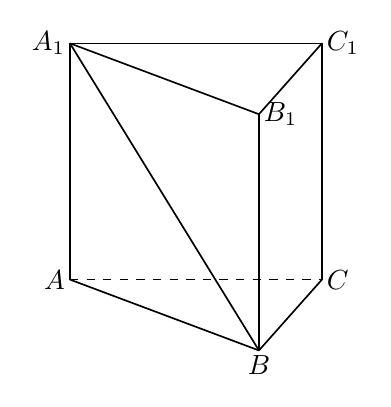
\begin{tikzpicture}[scale=1.0, semithick, every node/.style={inner sep=1.5pt}]
  \coordinate (A) at (0.20,0.40);
  \coordinate (C) at (3.40,0.40);
  \coordinate (B) at (2.60,-0.50);
  \coordinate (A1) at (0.20,3.40);
  \coordinate (C1) at (3.40,3.40);
  \coordinate (B1) at (2.60,2.50);

  \draw (A1) -- (C1);
  \draw (A1) -- (B1);
  \draw (B1) -- (C1);
  \draw (A) -- (A1);
  \draw (B) -- (B1);
  \draw (C) -- (C1);
  \draw (A) -- (B);
  \draw (B) -- (C);
  \draw (A1) -- (B);
  \draw[dashed] (A) -- (C);

  \node[left] at (A) {$A$};
  \node[below] at (B) {$B$};
  \node[right] at (C) {$C$};
  \node[left] at (A1) {$A_1$};
  \node[right] at (B1) {$B_1$};
  \node[right] at (C1) {$C_1$};
\end{tikzpicture}
\end{center}
\nopagebreak[4]
\Needspace{0.4\textheight}
\end{question}
\begin{question}
\gkti{19}如图，要设计一张矩形广告，该广告含有大小相等的左右两个矩形栏目（即图中阴影部分），这两栏的面积之和为 $18000$ cm²，四周空白的宽度为 $10$ cm，两栏之间的中缝空白的宽度为 $5$ cm，怎样确定广告的高与宽的尺寸（单位：cm），能使矩形广告面积最小？
\nopagebreak[4]
\begin{center}% 2008 年湖北卷文科第 19 题：矩形广告版式示意——左右两个大小相等的矩形栏目（阴影），
%   四周空白宽 10 cm，中缝空白宽 5 cm。
% 来源 PDF：gaokaomath-src/普通高考/2008/2008湖北文.pdf
% SHA-256：e097163e244cb8f03775ac7ff2e344ef85471e91ecc717d23698a0fb01e76963
% 原页：2008湖北文.pdf 第 2 页（A3 三栏）第 1 栏，书页码 452。
% 重绘依据：按原页画外框矩形，内部两个等宽阴影矩形，左右与上下留边等宽，两栏之间留中缝。
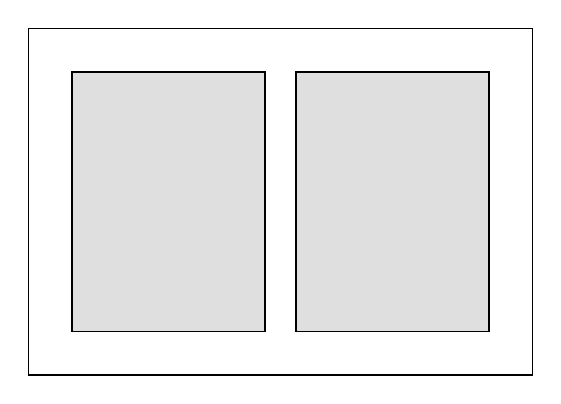
\begin{tikzpicture}[x=1.0cm, y=1.0cm, semithick]
  % 外框
  \draw (0,0) rectangle (6.4,4.4);
  % 两个栏目
  \fill[gray!25] (0.55,0.55) rectangle (3.00,3.85);
  \fill[gray!25] (3.40,0.55) rectangle (5.85,3.85);
  \draw (0.55,0.55) rectangle (3.00,3.85);
  \draw (3.40,0.55) rectangle (5.85,3.85);
\end{tikzpicture}
\end{center}
\nopagebreak[4]
\end{question}
\begin{question}
\gkti{20}已知双曲线 $C$：$\dfrac{x^2}{a^2}-\dfrac{y^2}{b^2}=1$（$a>0$，$b>0$）的两个焦点为 $F_1(-2,0)$，$F_2(2,0)$，点 $P(3,\sqrt7)$ 在双曲线 $C$ 上。

（1）求双曲线 $C$ 的方程；

（2）记 $O$ 为坐标原点，过点 $Q(0,2)$ 的直线 $l$ 与双曲线 $C$ 相交于不同的两点 $E$、$F$，若 $\triangle OEF$ 的面积为 $2\sqrt2$，求直线 $l$ 的方程。

\end{question}
\begin{question}
\gkti{21}已知数列 $\{a_n\}$ 和 $\{b_n\}$ 满足：$a_1=\lambda$，$a_{n+1}=\dfrac23a_n+n-4$，$b_n=(-1)^n(a_n-3n+21)$，其中 $\lambda$ 为实数，$n$ 为正整数。

（1）证明：对任意实数 $\lambda$，数列 $\{a_n\}$ 不是等比数列；

（2）证明：当 $\lambda\neq-18$ 时，数列 $\{b_n\}$ 是等比数列；

（2）设 $S_n$ 为数列 $\{b_n\}$ 的前 $n$ 项和，是否存在实数 $\lambda$，使得对任意正整数 $n$，都有 $S_n>-12$？若存在，求 $\lambda$ 的取值范围；若不存在，说明理由。

\end{question}